\documentclass[name = Quiz]{homework}

\usepackage{caption, subcaption, pdfpages, float}
\usepackage{graphics, wrapfig, pgf, graphicx}
\usepackage{enumitem}


% pacotes para importar código
\usepackage{caption, booktabs}
\usepackage[inkscapepath=build/inkscape]{svg}
\usepackage[section, newfloat, outputdir=build/]{minted}
\definecolor{sepia}{RGB}{252,246,226}
\setminted{
    bgcolor = sepia,
    style   = pastie,
    frame   = leftline,
    autogobble,
    samepage,
    python3,
    breaklines
}
\setmintedinline{
    bgcolor={}
}

% ambientes de códigos de Python
\newmintedfile[pyinclude]{python3}{}
\newmintinline[pyline]{python3}{}
\newcommand{\pyref}[2]{\href{#1}{\texttt{#2}}}

% \SetupFloatingEnvironment{listing}{name=Código}
% \captionsetup[listing]{position=below,skip=-1pt}

\usepackage{csquotes}
\usepackage[
    style    = verbose-ibid,
    autocite = footnote,
    notetype = foot+end,
    backend  = biber
]{biblatex}
\addbibresource{references.bib}
\usepackage[section]{placeins}

\usepackage[hidelinks]{hyperref}
\usepackage[noabbrev, nameinlink]{cleveref}
\hypersetup{
    pdftitle  = {MO412/MC908 - RA187679},
    pdfauthor = {Tiago de Paula}
}

\newcommand{\textref}[2]{
    \hyperref[#2]{#1 \ref*{#2}}
}

\renewcommand{\vec}[1]{\mathbf{#1}}

\DeclareMathOperator{\round}{round}

\usepackage{import, multirow}
\usepackage{pgf, tikz}
\usetikzlibrary{matrix}
\usetikzlibrary{positioning}
\usetikzlibrary{automata}
\usetikzlibrary{shapes}

\usepackage{wrapfig}
\usepackage{booktabs}
\usepackage{enumitem}
\usepackage{multicol}
\usepackage{physics}
\usepackage{amsmath, amssymb, bm, mathtools}
\usepackage{etoolbox, xpatch, xspace}
% \usepackage[mathcal]{euscript}
% \usepackage[scr]{rsfso}
% \usepackage{mathptmx}
\usepackage{relsize, centernot}
\usepackage{physics}


\makeatletter

% %% Símbolo QED %%
% \renewcommand{\qedsymbol}{\ensuremath{\mathsmaller\blacksquare}}

%% Marcadores de Prova: \direto, \inverso %%
\newcommand{\direto}[1][~]{\ensuremath{(\rightarrow)}#1\xspace}
\newcommand{\inverso}[1][~]{\ensuremath{(\leftarrow)}#1\xspace}

\undef\sum
%% Somatório: \sum_i^j, \bigsum_i^j %%
\DeclareSymbolFont{cmex10}{OMX}{cmex}{m}{n}
\DeclareMathSymbol{\sum@d}{\mathop}{cmex10}{"58}
\DeclareMathSymbol{\sum@t}{\mathop}{cmex10}{"50}
\DeclareMathOperator*{\sum}{\mathchoice{\sum@d}{\sum@t}{\sum@t}{\sum@t}}
\DeclareMathOperator*{\bigsum}{\mathlarger{\mathlarger{\sum@d}}}

%% Operadores de Conjunto: \pow(S), \Dom(S), \Img(S) %%
\DeclareSymbolFont{boondox}{U}{BOONDOX-cal}{m}{n}
\DeclareMathSymbol{\pow}{\mathalpha}{boondox}{"50}
\DeclareMathOperator{\Dom}{Dom}
\DeclareMathOperator{\Img}{Im}

\undef\Phi
%% Variantes gregas %%
\DeclareSymbolFont{cmr10}{OT1}{cmr}{m}{n}
\DeclareSymbolFont{cmmi10}{OML}{cmm}{m}{it}
\DeclareMathSymbol{\Phi}{\mathalpha}{cmr10}{"08}
\DeclareMathSymbol{\varpsi}{\mathalpha}{cmmi10}{"20}
\DeclareMathSymbol{\varomega}{\mathalpha}{cmmi10}{"21}

%% Família de Conjuntos: \family{S} %%
\DeclareMathAlphabet{\family}{OMS}{cmsy}{m}{n}

\undef\natural
\undef\real
%% Conjuntos Padrões: R, N, Z, C, Q %%
\DeclareMathOperator{\real}{\mathbb{R}}
\DeclareMathOperator{\natural}{\mathbb{N}}
\DeclareMathOperator{\integer}{\mathbb{Z}}
\DeclareMathOperator{\complex}{\mathbb{C}}
\DeclareMathOperator{\rational}{\mathbb{Q}}

%% Definição de Conjuntos: \set{ _ \mid _ } %%
\newcommand{\set}[1]{%
    \begingroup%
        \def\mid{\;\middle|\;}%
        \left\{#1\right\}
    \endgroup%
}

%% Novos Operadores: \modulo, \symdif, \grau %%
\DeclareMathOperator{\modulo}{~mod~}
\DeclareMathOperator{\symdif}{\mathrel{\triangle}}
\DeclareMathOperator{\grau}{deg}

%% Operadores Delimitados: \abs{\sum_i^j}, x \equiv y \emod{n} %%
% \newcommand{\abs}[1]{{\left\lvert\,#1\,\right\rvert}}
\newcommand{\emod}[1]{\ \left(\mathrm{mod}\ #1\right)}

%% Vérices e Arestas %%
\DeclareMathOperator{\Adj}{Adj}
\DeclareMathOperator{\dist}{dist}

\makeatother


\newenvironment{kmatrix}[1][1.3cm]{
    \begin{tikzpicture}[node distance=0cm]
        \tikzset{square matrix/.style={
                matrix of nodes,
                column sep=-\pgflinewidth, row sep=-\pgflinewidth,
                nodes={draw,
                    minimum height=#1,
                    anchor=center,
                    text width=#1,
                    align=center,
                    inner sep=0pt
                },
            },
            square matrix/.default=#1
        }
}{
    \end{tikzpicture}%
}

\newcommand*{\Scale}[2][4]{\scalebox{#1}{\ensuremath{#2}}}%

\newcommand{\red}[1]{\textcolor{red}{\textbf{#1}}}
\def\qm{?}

\newcommand{\quiz}[2]{\section*{\href{#2}{#1}}}

\begin{document}
    \pagestyle{main}

    For each question, give the answer and a short justification.

    \quiz{2021-013}{https://net-sci-questions.blogspot.com/2021/03/2021-013.html}

Choose the option that contains the derivative of $f(x) = g(x) h(x)$, where $g(x) = x^3$ and $h(x) = (1 + \ln x)^2$.

\begin{enumerate}[label={\Alph*.}]
    \item $3x^2 + 2 (1 + \ln x)/x$
    \item $x^2 (1 + \ln x) (5 + \ln x)$
    \item $x^2 (1 + \ln x) (5 + 3 \ln x)$
    \item $x^2 (1 + \ln x) (5 + 3 \ln x + 2x)$
    \item None of the above
\end{enumerate}

Original idea by: Maria Tejada Begazo
 \newpage
    \quiz{2021-018}{https://net-sci-questions.blogspot.com/2021/04/2021-018.html}

Suppose that we want to build an \textbf{undirected network} with \textbf{200 nodes} and \textbf{600 links}. What will the \textit{average degree} of this network be?

\begin{enumerate}[label={\Alph*.}]
    \item 5
    \item 6
    \item 7
    \item 8
    \item None of the above
\end{enumerate}

Original idea by: Hismael Costa
 \newpage
    \quiz{2021-036}{https://net-sci-questions.blogspot.com/2021/06/2021-036.html}

Consider a Random Network such that $N = 1000$ and $p = 0.004$. We need to break apart its giant component, and the only way to do that is by randomly removing nodes. Under these conditions, how many nodes should we remove at minimum to have a good chance of achieving our goal?

\begin{enumerate}[label={\Alph*.}]
    \item 750
    \item 720
    \item 840
    \item 810
    \item None of the above
\end{enumerate}

Original idea by: José Nascimento


\subsection*{Answer: A}

Using the Binomal distribution, we have \[
    \langle k \rangle = p (N - 1) = 3.996
\] And \[
    \left\langle k^2 \right\rangle = p (1-p) (N-1) + p^2 (N-1)^2 = 19.948
\]

Therefore, the critical threshold as given by the Molloy-Reed criterion is
\begin{align*}
    f_c &= 1 - \frac{1}{\frac{\left\langle k^2 \right\rangle}{\left\langle k \right\rangle} - 1} \\
    &= 1 - \frac{1}{\frac{19.948}{3.996} - 1} \\
    &= 0.7495
\end{align*}

Then the giant component should start to break apart after $f_c \cdot N = 749.5$ nodes are removed.
 \newpage
    \quiz{2021-062}{https://net-sci-questions.blogspot.com/2021/10/2021-062.html}

Given two networks G1 and G2 generated by the Barabási-Albert model with $N = 1000$ and $N = 100$ nodes, respectively, find out which network likely has the smallest diameter. Also, give their expected diameters, rounded to two decimal places.

\begin{enumerate}[label={\Alph*.}]
    \item G1 has the smallest diameter, 6.29, while G2 has diameter 6.64
    \item G2 has the smallest diameter, 3.02, while G1 has diameter 3.57
    \item G1 has the smallest diameter, 3.22, while G2 has diameter 5.44
    \item G2 has the smallest diameter, 5.31, while G1 has diameter 5.44
    \item None of the above
\end{enumerate}

Original idea by: Victor Antonio Menuzzo
 \newpage
    \quiz{2022-082}{https://net-sci-questions.blogspot.com/2022/04/2022-082.html}

Considering that the evolution of a random network could be classified into four topologically distinct regimes, analyze the information below about a random network with N=1000 during different stages of its life.

\begin{enumerate}[label=\textbf{Stage \Roman*:}, leftmargin=*]
    \item p = 0.01
    \item p = 0.0036
    \item p = 0.001
    \item p = 0.0007
    \item p = 0.007
\end{enumerate}

Please, select the option that better represents the stage's topological regimes:

\begin{enumerate}[
    label = {\Alph*.},
    itemsep = 4\itemsep
]

\raggedcolumns\begin{multicols}{2}
    \item \begin{enumerate}[label=\textbf{Stage \Roman*:}, leftmargin=*]
        \item Connected
        \item Critical
        \item Subcritical
        \item Critical
        \item Connected
    \end{enumerate}

    \item \begin{enumerate}[label=\textbf{Stage \Roman*:}, leftmargin=*]
        \item Connected
        \item Connected
        \item Critical
        \item Subcritical
        \item Connected
    \end{enumerate}
\end{multicols}

\raggedcolumns\begin{multicols}{2}
    \item \begin{enumerate}[label=\textbf{Stage \Roman*:}, leftmargin=*]
        \item Connected
        \item Critical
        \item Subcritical
        \item Subcritical
        \item Supercritical
    \end{enumerate}

    \item \begin{enumerate}[label=\textbf{Stage \Roman*:}, leftmargin=*]
        \item Connected
        \item Supercritical
        \item Critical
        \item Subcritical
        \item Connected
    \end{enumerate}
\end{multicols}

    \item None of the above
\end{enumerate}

Original idea by: Felipe Crispim da Rocha Salvagnini


\subsection*{Answer: D}

Note that \[
    \langle k \rangle
        = \frac{2 \langle L \rangle}{N}
        = \frac{2 \cdot p L_{\max}}{N}
        = \frac{2 p}{N} \cdot \frac{N (N - 1)}{2}
        = p (N - 1)
\]

With that, we can fill the following table to analyze each stage:

\begin{table}[H]
    \centering
    \begin{tabular}{cccccc}
        \toprule
        Stage & $p$ & $\langle k \rangle = 999 p$ & Comp. to 1 & Comp. to $\ln N \approx 6.907$ & Regime \\
        \midrule\midrule
        I   & 0.01   & 9.99   & $\langle k \rangle > 1$       & $\langle k \rangle > 7 > \ln 1000$ & Connected \\
        II  & 0.0036 & 3.5964 & $\langle k \rangle > 1$       & $\ln 1000 > 6 > 3.5964$ & Supercritical \\
        III & 0.001  & 0.999  & $\langle k \rangle \approx 1$ & --- & Critical or Sub \\
        IV  & 0.0007 & 0.6993 & $1 > \langle k \rangle$       & --- & Subcritical\\
        V   & 0.007  & 6.993  & $\langle k \rangle > 1$       & $\langle k \rangle \approx \ln 1000$ & Super or Connected \\
        \bottomrule
    \end{tabular}
\end{table}

Since Stage II can only be Supercritical the only viable option  is D, which matches the other regimes.
 \newpage
    \quiz{2022-094}{https://net-sci-questions.blogspot.com/2022/04/2022-094.html}

A cell has an initial amount of $l_0$ liters of water inside it. After one hour has passed, the amount of water is $3 l_0 / 4$. If the rate of water usage for the cell's physiological functions is inversely proportional to the amount of water in the cell, find an equation that allows you to calculate the amount $L(t)$ of water in the cell at any point $t$ in time.

Note: Always consider positive values. Consider time measured in hours, and volume in liters.

\begin{enumerate}[label={\Alph*.}]
    \item $L(t) = l_0 \sqrt{16 - 7t} / 4$
    \item $L(t) = l_0 (4 - t) / 4$
    \item $L(t) = l_0 \sqrt{-7 t^2/16 + 1} / 4$
    \item $L(t) = l_0 (t^2 + 16) / 4$
    \item None of the above
\end{enumerate}

Original Idea by Rómulo Condori


\subsection*{Answer: A}

\setlength{\columnseprule}{0.4pt}
\raggedcolumns\begin{multicols}{2}
    By the problem description, \[
        \pdv{t} L(t) \propto \frac{1}{L(t)}
    \]

    That is, for some real $k$,
    \begin{align*}
        \pdv{L}{t} &= k \frac{1}{L} \\
        k &= L \dv{L}{t}
    \end{align*}

    If we integrate in $t$, we get
    \begin{align*}
        \int_0^t k \dd{t} &= \int_0^t L \pdv{L}{t} \dd{t} \\
        k t &= \int_{l_0}^{L(t)} L \dd{L} \\
        k t &= \eval{\frac{L^2}{2}}_{l_0}^{L(t)} \\
        k t &= \frac{L(t)^2 - l_0^2}{2}
    \end{align*}

    Such that \[
        L(t) = \sqrt{2 k t + l_0^2}
    \]

    As specified, at $t = 1 \text{h}$, $L(1) = 3 l_0 / 4$, therefore
    \begin{align*}
        L(1) = \sqrt{2 k + l_0^2} &= \frac{3 l_0}{4} \\
            2 k + l_0^2 &= \frac{9 l_0^2}{16} \\
            32 k + 16 l_0^2 &= 9 l_0^2 \\
            32 k + 7 l_0^2 &= 0 \\
            k &= - \frac{7}{32} l_0^2
    \end{align*}

    Then \begin{align*}
        L(t) &= \sqrt{- \frac{2 \cdot 7}{32} l_0^2 t + l_0^2} \\
            &= l_0 \sqrt{- \frac{7}{16} t + 1} \\
            &= l_0 \frac{\sqrt{- 7 t + 16}}{\sqrt{16}} \\
            &= \frac{l_0}{4} \sqrt{16 - 7 t}
    \end{align*}
\end{multicols}
\setlength{\columnseprule}{0pt}
 \newpage
    \quiz{2022-119}{https://net-sci-questions.blogspot.com/2022/05/2022-099.htmll}

Starting from the node indicated as `start', use DFS and label the nodes with their ending times. Which of the alternatives below corresponds to a possible answer?

\begin{figure}[H]
    \centering
    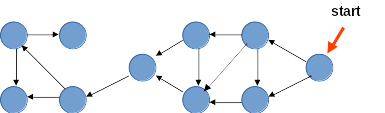
\includegraphics{images/119-0.png}
\end{figure}

Tip: the reverse order of finishing DFS times in a directed acyclic graph is a topological order.

\begin{enumerate}[label={\Alph*.}]

\raggedcolumns\begin{multicols}{2}
    \item 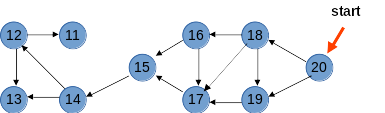
\includegraphics[width=0.45\textwidth]{images/119-A.png}

    \item 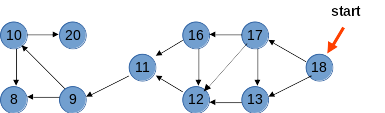
\includegraphics[width=0.45\textwidth]{images/119-B.png}
\end{multicols}

\raggedcolumns\begin{multicols}{2}
    \item 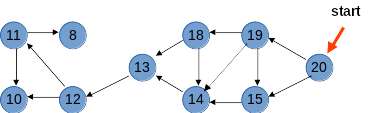
\includegraphics[width=0.45\textwidth]{images/119-C.png}

    \item 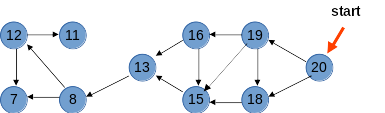
\includegraphics[width=0.45\textwidth]{images/119-D.png}
\end{multicols}

    \item None of the above
\end{enumerate}

Original ideia by: Filipe Maciel Roberto


\subsection*{Answer: C}

The given digraph is acyclic, therefore the finishing time must form a topological sorting of its vertices.

For \textbf{A.}, we have 18 as a successor to 19 in the topological order, but there's a back arc from 18 to 19, invalidating this order.

For \textbf{B.}, there's an arc from 10 to 20. In fact, the start node is the last to finish and  must have the largest finishing time.

For \textbf{C.}, the topological order is valid:

\begin{figure}[H]
    \centering
    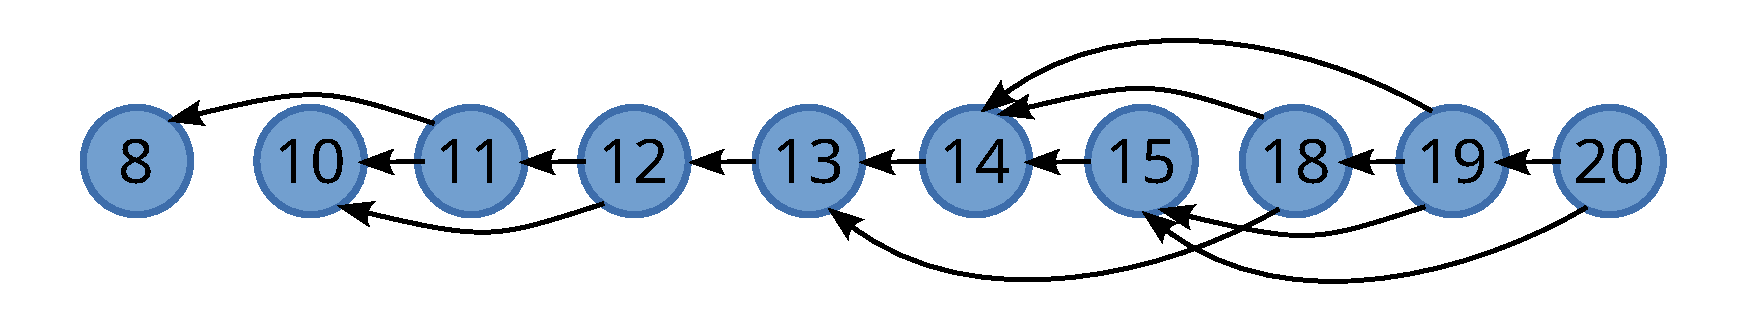
\includegraphics[width=0.95\textwidth]{images/119.pdf}
\end{figure}

For \textbf{D.}, the single invalid arc is from 8 to 12.
 \newpage
    \quiz{2022-130}{https://net-sci-questions.blogspot.com/2022/06/2022-130.html}

Consider the following statements about degree correlation in networks:

\begin{enumerate}[label={\Roman*.}]
    \item In neutral networks, nodes link to each other randomly, which in turn results in a lack of degree correlation for the linking pattern.
    \item A perfectly assortative network is always a complete graph.
    \item The correlation exponent can help determine the type of the network. When the correlation exponent is positive, we may say the network is assortative.
    \item In assortative networks, nodes tend to link to nodes of similar degree. In other words, hubs tend to connect with hubs, and small-degree nodes tend to connect with small-degree nodes.
    \item Degree correlations for directed network's are defined by two coefficients: $r_{\text{in},\text{out}}$ and $r_{\text{out},\text{in}}$.
\end{enumerate}

Select the alternative that lists the correct statements:

\begin{enumerate}[label={\Alph*.}]
    \item I, II, and V are correct.
    \item Only V is correct.
    \item II, III, and IV are correct.
    \item I, II, III, and IV are correct.
    \item None of the above.
\end{enumerate}

Original idea by: Heitor Mattosinho


\end{document}
